\begin{table}[H]
\centering
\definecolor{tabglobalcrossb0}{rgb}{0.9961,0.725,0.3271}
\definecolor{tabglobalcrossb1}{rgb}{0.995,0.6599,0.2816}
\definecolor{tabglobalcrossb2}{rgb}{0.99,0.4173,0.1965}
\definecolor{tabglobalcrossb3}{rgb}{0.9915,0.5103,0.2231}
\definecolor{tabglobalcrossb4}{rgb}{0.9885,0.3243,0.17}
\definecolor{tabglobalcrossb5}{rgb}{0.891,0.1036,0.1102}
\definecolor{tabglobalcrossb6}{rgb}{0.9617,0.2507,0.1499}
\definecolor{tabglobalcrossb7}{rgb}{0.6821,0.0,0.149}
\definecolor{tabglobalcrossb8}{rgb}{0.502,0.0,0.149}
\definecolor{tabglobalcrossb9}{rgb}{0.854,0.0772,0.1193}
\definecolor{tabglobalcrossb10}{rgb}{0.5845,0.0,0.149}
\definecolor{tabglobalcrossb11}{rgb}{0.547,0.0,0.149}
\definecolor{tabglobalcrossb12}{rgb}{0.8773,0.0932,0.1132}
\definecolor{tabglobalcrossb13}{rgb}{0.8446,0.0708,0.1218}
\definecolor{tabglobalcrossb14}{rgb}{0.7511,0.0068,0.1464}
\definecolor{tabglobalcrossb15}{rgb}{0.8586,0.0804,0.1181}
\definecolor{tabglobalcrossb16}{rgb}{0.9217,0.1675,0.1275}
\definecolor{tabglobalcrossb17}{rgb}{0.607,0.0,0.149}
\definecolor{tabglobalcrossb18}{rgb}{0.9371,0.1995,0.1361}
\definecolor{tabglobalcrossb19}{rgb}{1.0,0.9801,0.7513}
\definecolor{tabglobalcrossb20}{rgb}{1.0,0.9402,0.6538}
\definecolor{tabglobalcrossb21}{rgb}{0.9984,0.8971,0.5596}
\definecolor{tabglobalcrossb22}{rgb}{0.9961,0.8498,0.4615}
\definecolor{tabglobalcrossb23}{rgb}{0.9961,0.7634,0.3684}
\definecolor{tabglobalcrossb24}{rgb}{0.9955,0.6781,0.2894}
\definecolor{tabglobalcrossb25}{rgb}{0.9933,0.5962,0.254}
\definecolor{tabglobalcrossb26}{rgb}{0.991,0.4793,0.2143}
\definecolor{tabglobalcrossb27}{rgb}{0.9888,0.3398,0.1744}
\definecolor{tabglobalcrossb28}{rgb}{0.9463,0.2187,0.1412}
\definecolor{tabglobalcrossb29}{rgb}{0.8867,0.0996,0.1107}
\definecolor{tabglobalcrossb30}{rgb}{0.8025,0.042,0.1329}
\definecolor{tabglobalcrossb31}{rgb}{0.7046,0.0,0.149}
\definecolor{tabglobalcrossb32}{rgb}{0.5695,0.0,0.149}
\begin{minipage}{0.78\textwidth}
\centering
\renewcommand{\arraystretch}{1.2}
\begin{tabular}{lccc}
\toprule
Checkpoint & First & Middle & Last \\
\midrule
0 & \cellcolor{tabglobalcrossb0}\textcolor{black}{$0.082 \pm 0.030$} & \cellcolor{tabglobalcrossb1}\textcolor{black}{$0.095 \pm 0.015$} & \cellcolor{tabglobalcrossb2}\textcolor{black}{$0.132 \pm 0.025$} \\
1 & \cellcolor{tabglobalcrossb3}\textcolor{black}{$0.121 \pm 0.026$} & \cellcolor{tabglobalcrossb4}\textcolor{white}{$0.143 \pm 0.035$} & \cellcolor{tabglobalcrossb5}\textcolor{white}{$0.174 \pm 0.033$} \\
5 & \cellcolor{tabglobalcrossb6}\textcolor{white}{$0.153 \pm 0.033$} & \cellcolor{tabglobalcrossb7}\textcolor{white}{$0.210 \pm 0.055$} & \cellcolor{tabglobalcrossb8}\textcolor{white}{$0.232 \pm 0.051$} \\
15 & \cellcolor{tabglobalcrossb9}\textcolor{white}{$0.181 \pm 0.038$} & \cellcolor{tabglobalcrossb10}\textcolor{white}{$0.222 \pm 0.036$} & \cellcolor{tabglobalcrossb11}\textcolor{white}{$0.227 \pm 0.021$} \\
50 & \cellcolor{tabglobalcrossb12}\textcolor{white}{$0.176 \pm 0.027$} & \cellcolor{tabglobalcrossb13}\textcolor{white}{$0.183 \pm 0.022$} & \cellcolor{tabglobalcrossb14}\textcolor{white}{$0.201 \pm 0.017$} \\
200 & \cellcolor{tabglobalcrossb15}\textcolor{white}{$0.180 \pm 0.030$} & \cellcolor{tabglobalcrossb16}\textcolor{white}{$0.165 \pm 0.014$} & \cellcolor{tabglobalcrossb17}\textcolor{white}{$0.220 \pm 0.029$} \\
last & \cellcolor{tabglobalcrossb5}\textcolor{white}{$0.173 \pm 0.025$} & \cellcolor{tabglobalcrossb18}\textcolor{white}{$0.160 \pm 0.012$} & \cellcolor{tabglobalcrossb8}\textcolor{white}{$0.232 \pm 0.037$} \\
\bottomrule
\end{tabular}
\end{minipage}%
\hfill
\begin{minipage}{0.15\textwidth}
\centering
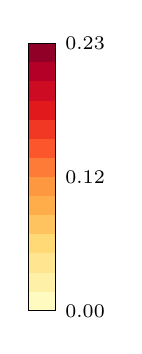
\begin{tikzpicture}
\fill[tabglobalcrossb19] (0,0.0000) rectangle (0.35,0.2429);
\fill[tabglobalcrossb20] (0,0.2429) rectangle (0.35,0.4857);
\fill[tabglobalcrossb21] (0,0.4857) rectangle (0.35,0.7286);
\fill[tabglobalcrossb22] (0,0.7286) rectangle (0.35,0.9714);
\fill[tabglobalcrossb23] (0,0.9714) rectangle (0.35,1.2143);
\fill[tabglobalcrossb24] (0,1.2143) rectangle (0.35,1.4571);
\fill[tabglobalcrossb25] (0,1.4571) rectangle (0.35,1.7000);
\fill[tabglobalcrossb26] (0,1.7000) rectangle (0.35,1.9429);
\fill[tabglobalcrossb27] (0,1.9429) rectangle (0.35,2.1857);
\fill[tabglobalcrossb28] (0,2.1857) rectangle (0.35,2.4286);
\fill[tabglobalcrossb29] (0,2.4286) rectangle (0.35,2.6714);
\fill[tabglobalcrossb30] (0,2.6714) rectangle (0.35,2.9143);
\fill[tabglobalcrossb31] (0,2.9143) rectangle (0.35,3.1571);
\fill[tabglobalcrossb32] (0,3.1571) rectangle (0.35,3.4000);
\draw[black,line width=0.3pt] (0,0) rectangle (0.35,3.4000);
\node[right,font=\scriptsize,anchor=west] at (0.35,3.4000) {0.23};
\node[right,font=\scriptsize,anchor=west] at (0.35,1.7000) {0.12};
\node[right,font=\scriptsize,anchor=west] at (0.35,0) {0.00};
\end{tikzpicture}
\end{minipage}
\caption{Global cross-comparison, Direction B (both unnormalised, different training objective). Mean $\pm$ SE across 10 datasets (First/Last), 8 for Middle (datasets with $L=2$ contribute no middle layer). (Pooled fold/layer SE averages 0.010 across cells; not shown per cell, see text.) Cell shading: white = 0, dark red = 0.23 (max value in this table), YlOrRd colormap, same scale as Fig.~\ref{fig: RM_Norm} etc.}
\label{tab:global_cross_b}
\end{table}
